% The difference between quantum and classical mechanics does not involve just a small tweak. Instead it is a root and branch overhaul of the entire framework.\par
量子力学与经典力学的不同不是一点两点。相反,它是对整个物理框架的彻底改革。\par
% This is manifest from the very beginning as we can see by comparing how we describe the state of a system in the two frameworks. The state is the information that tells us all we need to know about the system at a fixed time, with the idea that the laws of physics will then dictate how the state evolves at all later times. Throughout these lectures we will deal only with the dynamics of a single particle. For the present discussion, we’ll think about a particle moving in $\mathbf{R}^3$\par
这一点从一开始就很明显,我们可以通过比较在两种框架下描述系统状态的方式看出。状态可以告诉我们某时刻系统的所有信息,通过物理定律,我们可以算出接下去每一时刻的系统的状态。 在接下去的课程中,我们只处理单个粒子的运动。就现在的讨论,我们只考虑在$\mathbf{R}^3$空间中运动的粒子。\par
% In the classical world, the state of the particle is determined by its position x and its velocity $\mathbf{v}=\dot{\mathbf{x}}$. If you specify both bits of information at some time $t_0$ then you can use the equation of motion $\mathbf{F} = m\ddot{\mathbf{x}}$ to determine $\mathbf{x}(t)$ and $\mathbf{v}(t)$ for all time. Importantly, it’s not enough to just know only, say, the position of the particle at $t = t_0$. You need both $\mathbf{x}(t_0)$ and $\mathbf{v}(t_0)$. Mathematically, this is because the equation of motion is a second order differential equation and so you need to specify two integration constants to get a unique solution.\par
在经典物理中,粒子的状态只由它的位置$\mathbf{x}$和它的速度$\mathbf{v}=\dot{\mathbf{x}}$决定。如果你在某个时间$t_0$知道这两个信息,那么你可以使用运动方程$\mathbf{F} = m\ddot{\mathbf{x}}$来确定接下去所有时间的$\mathbf{x}(t)$和$\mathbf{v}(t)$。
% In the quantum world, the state of a particle is determined by its wavefunction. This is a complex valued function
在量子世界中质点的状态,只由它的波函数确定。这是一个复值函数
\[
    \psi(\mathbf{x},t)
\]
% As we will see, if you know the wavefunction at some time, say $t_0$, then you have all the information that you need to determine the state at all other times.\par
我们将会看见,如果你知道某时刻$t_0$的波函数,那么你就可以得到之后所有时间确定状态所需的所有信息.\par
% The description in terms of the wavefunction is not a small amendment to classical mechanics. We’ve replaced the three position coordinates $\mathbf{x}\in \mathbf{R}^3$ with an infinite amount of information, a functions worth of information. Moreover, we haven’t speci- fied anything about the particle’s velocity; that information must also be contained, in some manner, in the wavefunction $\psi(\mathbf{x},t)$.\par
用波函数描述系统与经典力学截然不同。我们已经将三个位置坐标$\mathbf{x}\in \mathbf{R}^3$用一个有着无限有用信息的函数替代。此外,我们还没有说明粒子的速度;这个信息必须以某种方式包含在$\psi(\mathbf{x},t)$中。\par
% The wavefunction has a very simple interpretation. Or, more precisely, the modsquare of the wavefunction has a very simple interpretation. It tells us the probability that we will find a particle at a given position. The probability density $P$ for a particle to sit at point $\mathbf{x}$ is
波函数有一种非常简单的解释,或者说波函数的模方有一个非常简单的解释。 他告诉我们粒子出现在某一个位置的概率。粒子出现在$\mathbf{x}$处的概率$P$是
\[
P(\mathbf{x},t) =|\psi(\mathbf{x},t)|^2
\]
% This is known as the Born rule, after Max Born who first understood that quantum mechanics is a theory of probability rather than certainty.\par
这被称作\textit{Born定则}, Max Born 第一次意识到量子理论是一个概率的理论,而不是确定的理论。\par
% From the probability density, you can compute actual probabilities by multiplying by a volume: the probability that the particle sits in some small volume $\mathrm{d}V$ centred around point $\mathbf{x}$ is $P(\mathbf{x},t)\mathrm{d}V$ .\par
从概率密度的角度来说,你可以将概率密度乘上体积来计算粒子出现在某个小体积$\mathrm{d}V$中心附近的概率,其概率为$P(\mathbf{x},t)\mathrm{d}V$。\par
% In all other realms of science, probability arises because of our ignorance. If you throw a classical dice, and know its initial state with complete precision, then there is no doubt about what will happen. Once the dice leaves your hand, the probability that you will roll a six is either 0 or 1. If you were really good at solving differential equations, you could just figure out the answer and impress your friends. But, in most circumstances we don’t have a good knowledge of the initial state of the dice and, besides, differential equations are hard. So we just give up, admit that we don’t know what will happen, and say that the probability of rolling a six is $\frac{1}{6}$. Crucially, however,the introduction of probability is entirely due to our lack of knowledge; it is not an inherent property of the dice.\par
在所有其他的科学领域中概率的产生,是由于我们的不了解。 如果你扔一个骰子,并且完全精确地知道它的初始状态,那接下去会发生什么就毫无疑义了。 你可以扔到六点的概率不是0就是1。 如果你非常善于解微分方程,你可以就算出答案来震惊你的朋友。 但在绝大多数情况下,我们对初值条件的了解,并不是非常精确,另外,解微分方程非常困难。 所以我们放弃了,承认我们不知道将会发生什么,然后承认扔到六点的概率为$\frac{1}{6}$。 从上面的例子可以看出概率的来源,是因为我们对初值条件的不了解,而不是骰子本身的属性。
% This is not the case in quantum mechanics. The state $\psi(\mathbf{x},t)$ contains all the information about a particle and the probabilistic interpretation is not because of any failing on our part, but instead due to an inherent randomness in the quantum world. This is, to put it mildly, something of a departure from the Newtonian way of thinking.\par
但这与量子力学中不同。状态$\psi(\mathbf{x},t)$包含了关于一个粒子的所有信息,并且概率的产生不是由于我们的问题,而是量子世界内在的随机性。这与牛顿式的思考方式不同。
% The novelty in the wavefunction description of the particle might suggest other interpretations of the function $\psi(\mathbf{x},t)$. You might, for example, wonder if perhaps we shouldn’t think of a particle at all, but rather some fluid-like object, spread out over space. Such objects are commonplace in physics and are known as $fields$. The electric and magnetic fields are familiar examples. But that’s not the right way to think about the wavefunction. This is because we never observe a fragmented particle, one that’s lost its particle form and starts spreading jell-o like throughout space. Any measuring device that will allow you to determine whether a particle is in some designated region of space will return the answer yes or no. It won’t tell you “well, the particle’s a little bit here but mostly somewhere over there to the left”. The wavefunction doesn’t describe some real fluid; it is more nebulous. It is a wave only of probability.
用波函数描述粒子的这一种全新的方式,可能会给波函数$\psi(\mathbf{x},t)$带来不同的解释。比如说,我们根本不应该考虑质点, 而是空间分布像流体一样的分布的物体。 在物理中称之为\textit{场}。 电场和磁场是我们熟悉的例子. 但这\textit{不}是我们理解过函数的方式。 就是因为我们从来没有观测到过一个弥散的粒子,一个失去了粒子形式,开始像果冻一样在太空中扩散的粒子。任何让你确定一个粒子是否在某个区域的观测,只会返回是或者否。 观测不会告诉你,“这个粒子部分在这里,但大部分在其他地方。”波函数不能描述真实的流体;它更加模糊,只能表示概率。
\begin{figure}[h]
    \centering
    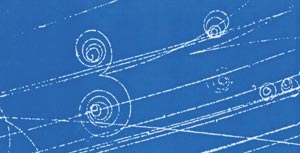
\includegraphics{img/1.jpg}
    % \caption{In any particular experiment, you only detect particles with very definite trajectories and no hint of the more nebulous underlying wavefunction.}
    \caption{在任何的实验中,只能检测到具有明确轨迹的粒子,而没有波函数的迹象}
    % \label{fig:mesh1}
\end{figure}\par
% This is illustrated in Figure 1 which shows the tracks left by electrons and positrons as they pass through a detector known as a bubble chamber. The fast travelling particles move in approximately straight lines, while those that are slower spiral in circles due to an applied magnetic field. The electrons bend one way, the positrons the other, giving the back-to-back spirals that you can see. For our purposes, the key point is that when the particles entered the detector, they were described by a wavefunction that was spread out over a large part of space. Yet, the particles don’t appear as fluffy, insubstantial clouds of probability. Instead, they leave clear tracks, with a definite trajectory.\par
图1显示了正电子和负电子穿过云室时的轨迹。 快速运动的粒子大约沿直线前进, 那些运动的比较慢的粒子,在磁场的作用下作螺旋运动。 电子向一个方向旋转,同时正电指向另一个方向旋转。 我们认为粒子进入探测器时,它们是由一个分布在很大空间中的波函数所描述的。 但是这些粒子并没有任何弥散的现象。 相反,他们有明确的轨迹。
% The introduction of probability at such a fundamental level means that we must abandon the idea of predicting, with certainty, what will happen in a given experiment. There is no way to say when and where the spirals will appear in the picture above. We can only compute the likelihood for this to happen. Clearly this is retrograde step from the Newtonian (strictly, Laplacian) dream of knowing everything that will happen, from the beginning to the end of time.\par
在如此基本的地方就引入概率,意味着我们必须要放弃精准预测的想法。 我们没有办法精准预测,在哪个地方会出现螺旋。 我们只能计算它的可能性。 显然这打破了Newton(准确来说,是Laplace)的梦想,即知道从开始到结束发生的一切。\par
% One might wonder if perhaps it’s possible to restore this dream at some deeper level. Maybe the wavefunction $\psi(\mathbf{x},t)$ is just some coarse-grained description of something finer and more subtle that’s going on underneath. Maybe another layer of reality awaits discovery, one that allows us to bring back our comfortable deterministic, Newtonian way of thinking. There is good reason to think that this is not the case. Reality is, at heart, probabilistic. We’ll mention some of the arguments for this in Section 3.5 where we touch upon some of the interpretations of quantum mechanics. A fuller description of why a deterministic world is incompatible with experiment will be given in the the lectures on Topics in Quantum Mechanics (see, in particular, the section on Quantum Foundations). For now, you’ll just have to accept that the world in which we live is not the one our forefathers grew up believing in. It is random and uncertain. It is also, as we will see, considerably more interesting because of it.
一些人可能会希望从更基本的地方来实现这一梦想。 可能波函数$\psi(\mathbf{x},t)$只是对接下去发生的更加精妙的事情的一个粗略的描述。 或者波函数有另一种解释,等待着我们去发现,让我们可以回到用更加舒适的Newton方法思考问题。 有充分的理由让我们不该这么做。 从本质上讲现实是概率的。 我们将在\S 3.5的时候遇到在这方面的讨论。 一个更加全面的描述为什么决定论的世界和实验是不相融的, 将会在量子力学专题研究\footnote{这是David Tong的另外一本讲义,可以在https://www.damtp.cam.ac.uk/user/tong/topicsinqm.html处找到——译者注}中描述(特别是在量子基本原理部分)。现在,你只能接受这一事实:我们生活的世界与我们的祖先从小所信仰的世界不同。它是随机和不确定的。我们将看到的,世界也因此变得有意思。

